\documentclass[tikz,crop,convert={density=200,outext=.png},border=0.4cm]{standalone}

\usepackage{pgfplots}
\usepackage{amsmath}
\usetikzlibrary{arrows.meta}
\usepackage{physics}
\usepackage{xcolor}
\definecolor{mixed_1}{RGB}{2,56,88}
\definecolor{mixed_2}{RGB}{54,144,192}
\definecolor{mixed_3}{RGB}{208,209,230}
\pgfplotsset{compat=newest,
    %width=6cm,
    %height=3cm,
    scale only axis=true,
    max space between ticks=25pt,
    try min ticks=5,
    every axis/.style={
        axis y line=middle,
        axis x line=middle,
        axis line style={thick,->,>=latex, shorten >=-.3cm}
    },
    every axis plot/.append style={thick},
    tick style={black, thick},
}
\tikzset{
    semithick/.style={line width=0.8pt},
}
\usepgfplotslibrary{groupplots}
\usepgfplotslibrary{dateplot}
% Document begins
\begin{document}
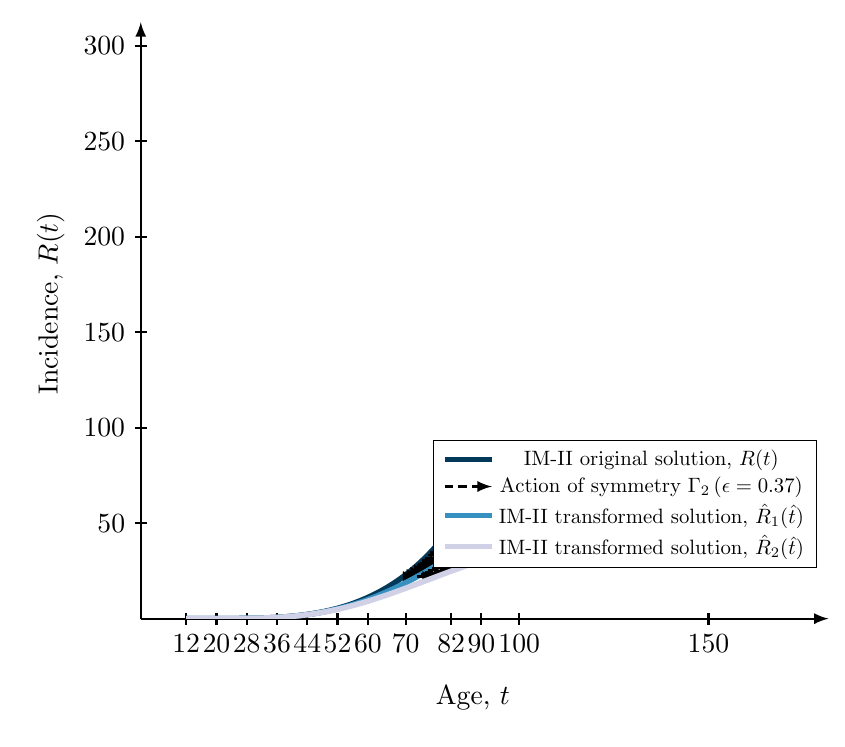
\begin{tikzpicture}
  % The axis of the plot
\begin{axis}[
    %title={Model: $\dv{y}{t}=\frac{2y}{t}$ with solution $y(t)=C_1t^2$\\Symmetry: $\Gamma_{\epsilon}=(t,y)\mapsto\left(\exp\left(\epsilon\right)t,\exp\left(-\epsilon\right)y\right)$},
    title style = {align=left},
    xlabel={Age, $t$},
    ylabel={Incidence, $R(t)$},
    %ylabel={Logarithm of Incidence, $\ln\left(R(t)\right)$},        
    x label style={at={(axis description cs:0.5,-0.1)},anchor=north},
    y label style={at={(axis description cs:-0.1,0.55)},rotate=90,anchor=south},    
    xmin=0, xmax=175.5,
    % xmin=-27, xmax=5,
    ymin=0, ymax=300,
    %xtick={-30,-27,...,9},
    xtick={0,12,20,...,60,70,82,90,100,150},    
    %ytick={-15,-10,...,15},
    legend style={at={(axis description cs:0.44,0.2)},anchor=west,nodes={scale=0.75, transform shape}},    
    %legend pos=north west,
    %ymajorgrids=true,
    grid style=dashed,
]
% Plot the data
\addplot[
color=mixed_1,line width=2pt,
]
coordinates {%
(12.0,0.0003931450378993812)
(12.717171717171716,0.0005588746263873061)
(13.434343434343434,0.0007858355258540312)
(14.151515151515152,0.0010933324841320433)
(14.868686868686869,0.0015056336609838839)
(15.585858585858585,0.0020529181568883907)
(16.303030303030305,0.0027723227724208177)
(17.02020202020202,0.003709080918415532)
(17.737373737373737,0.004917742612150893)
(18.454545454545453,0.006463460430219841)
(19.17171717171717,0.008423322333332697)
(19.88888888888889,0.01088770863388884)
(20.606060606060606,0.013961647246990106)
(21.32323232323232,0.017766138941657683)
(22.04040404040404,0.022439422759436195)
(22.757575757575758,0.02813815122467053)
(23.474747474747474,0.03503844552118372)
(24.19191919191919,0.04333680248749943)
(24.909090909090907,0.053250828063767)
(25.626262626262626,0.06501977562742947)
(26.343434343434343,0.07890487234686747)
(27.06060606060606,0.09518942208143906)
(27.77777777777778,0.11417867924467193)
(28.494949494949495,0.1361994941830517)
(29.21212121212121,0.16159973675404712)
(29.929292929292927,0.19074751066632914)
(30.646464646464644,0.22403017654310084)
(31.363636363636363,0.26185320638677734)
(32.08080808080808,0.30463889600015936)
(32.79797979797979,0.3528249648423879)
(33.515151515151516,0.4068630747034657)
(34.23232323232323,0.4672172994548196)
(34.94949494949495,0.534362578007944)
(35.666666666666664,0.6087831815621758)
(36.38383838383838,0.6909712243539333)
(37.101010101010104,0.7814252445657743)
(37.81818181818181,0.8806488789631804)
(38.535353535353536,0.9891496513555712)
(39.25252525252525,1.107437891279843)
(39.96969696969697,1.2360257955255376)
(40.686868686868685,1.3754266413917986)
(41.4040404040404,1.5261541570008228)
(42.12121212121212,1.6887220506826672)
(42.838383838383834,1.863643698462182)
(43.55555555555556,2.051431986069058)
(44.27272727272727,2.2525992996845337)
(44.98989898989899,2.467657657842836)
(45.707070707070706,2.6971189755159033)
(46.42424242424242,2.9414954504075683)
(47.14141414141414,3.201300060839202)
(47.858585858585855,3.477047164287253)
(48.57575757575757,3.7692531855938816)
(49.29292929292929,4.078437384072787)
(50.01010101010101,4.405122689131097)
(50.72727272727273,4.749836594583654)
(51.44444444444444,5.113112102510328)
(52.16161616161616,5.495488708264634)
(52.878787878787875,5.897513419052624)
(53.59595959595959,6.31974179933758)
(54.31313131313131,6.762739037166145)
(55.03030303030303,7.227081026336881)
(55.74747474747475,7.713355460128051)
(56.464646464646464,8.222162933057053)
(57.18181818181818,8.75411804785098)
(57.898989898989896,9.309850525461512)
(58.61616161616161,9.89000631655453)
(59.33333333333333,10.495248713444738)
(60.050505050505045,11.126259461928296)
(60.76767676767676,11.783739872894479)
(61.484848484848484,12.468411933972197)
(62.2020202020202,13.181019421793414)
(62.91919191919192,13.92232901573566)
(63.63636363636363,14.693131414244315)
(64.35353535353535,15.494242455036725)
(65.07070707070707,16.326504240656988)
(65.78787878787878,17.19078627098854)
(66.5050505050505,18.087986584442955)
(67.22222222222223,19.01903290963239)
(67.93939393939394,19.984883829403653)
(68.65656565656565,20.986529959165086)
(69.37373737373737,22.02499514147788)
(70.0909090909091,23.1013376589124)
(70.8080808080808,24.216651467191113)
(71.52525252525251,25.372067450652064)
(72.24242424242424,26.568754702075633)
(72.95959595959596,27.80792182892162)
(73.67676767676767,29.090818288025492)
(74.39393939393939,30.41873575080331)
(75.11111111111111,31.79300950101467)
(75.82828282828282,33.215019867134004)
(76.54545454545455,34.6861936913819)
(77.26262626262626,36.208005837470694)
(77.97979797979798,37.78198073912516)
(78.69696969696969,39.409693991444954)
(79.41414141414141,41.09277398718769)
(80.13131313131312,42.83290360006287)
(80.84848484848484,44.631821917145736)
(81.56565656565657,46.491326022537216)
(82.28282828282828,48.41327283442198)
(83.0,50.39958099770134)
};
\addlegendentry{IM-II original solution, $R(t)$}
\addplot[
color=black,->,>=latex,densely dashed
]
coordinates {%
(69.37373737373737,22.02499514147788)
(69.66787517748496,22.02499514147788)
(69.96940982337897,22.02499514147788)
(70.27867326786053,22.02499514147788)
(70.59601921581387,22.02499514147788)
(70.92182501908813,22.02499514147788)
(71.25649378439189,22.02499514147788)
(71.60045671872336,22.02499514147788)
(71.95417574500541,22.02499514147788)
(72.31814642594297,22.02499514147788)
(72.69290124049142,22.02499514147788)
(73.0790132649441,22.02499514147788)
};
\addlegendentry{Action of symmetry $\Gamma_{2}\left(\epsilon=0.37\right)$}
\addplot[
forget plot,
color=black,->,>=latex,densely dashed
]
coordinates {%
(70.0909090909091,23.1013376589124)
(70.40332896803592,23.1013376589124)
(70.72397780855756,23.1013376589124)
(71.0532428964987,23.1013376589124)
(71.39153816922497,23.1013376589124)
(71.73930666566821,23.1013376589124)
(72.09702325911614,23.1013376589124)
(72.46519771497302,23.1013376589124)
(72.8443781207327,23.1013376589124)
(73.23515474359404,23.1013376589124)
(73.63816438099617,23.1013376589124)
(74.05409528124896,23.1013376589124)
};
\addplot[
forget plot,
color=black,->,>=latex,densely dashed
]
coordinates {%
(70.8080808080808,24.216651467191113)
(71.13963476101182,24.216651467191113)
(71.48033030411128,24.216651467191113)
(71.83061841508822,24.216651467191113)
(72.19098266197793,24.216651467191113)
(72.56194235210138,24.216651467191113)
(72.94405606669282,24.216651467191113)
(73.33792563899233,24.216651467191113)
(73.74420064393699,24.216651467191113)
(74.16358348008467,24.216651467191113)
(74.5968351395939,24.216651467191113)
(75.04478178062855,24.216651467191113)
};
\addplot[
forget plot,
color=black,->,>=latex,densely dashed
]
coordinates {%
(71.52525252525251,25.372067450652064)
(71.87682066750551,25.372067450652064)
(72.23853027174556,25.372067450652064)
(72.61090553532179,25.372067450652064)
(72.99451041954127,25.372067450652064)
(73.38995269008606,25.372067450652064)
(73.79788847873891,25.372067450652064)
(74.21902744885945,25.372067450652064)
(74.65413866263582,25.372067450652064)
(75.10405726717656,25.372067450652064)
(75.56969213988855,25.372067450652064)
(76.0520346624561,25.372067450652064)
};
\addplot[
forget plot,
color=black,->,>=latex,densely dashed
]
coordinates {%
(72.24242424242424,26.568754702075633)
(72.61491561880342,26.568754702075633)
(72.99864282674001,26.568754702075633)
(73.39421412014853,26.568754702075633)
(73.80228617052263,26.568754702075633)
(74.22356923931221,26.568754702075633)
(74.6588330532114,26.568754702075633)
(75.10891349964558,26.568754702075633)
(75.57472028317848,26.568754702075633)
(76.05724571249516,26.568754702075633)
(76.55757482354973,26.568754702075633)
(77.07689708936002,26.568754702075633)
};
\addplot[
forget plot,
color=black,->,>=latex,densely dashed
]
coordinates {%
(72.95959595959596,27.80792182892162)
(73.35394940997857,27.80792182892162)
(73.76073536484155,27.80792182892162)
(74.18065845291608,27.80792182892162)
(74.6144821434299,27.80792182892162)
(75.06303535332704,27.80792182892162)
(75.52722000007566,27.80792182892162)
(76.0080196665269,27.80792182892162)
(76.50650957943864,27.80792182892162)
(77.0238681471664,27.80792182892162)
(77.56139035717314,27.80792182892162)
(78.12050340377348,27.80792182892162)
};
\addplot[
forget plot,
color=black,->,>=latex,densely dashed
]
coordinates {%
(73.67676767676767,29.090818288025492)
(74.09395274562506,29.090818288025492)
(74.52487769682638,29.090818288025492)
(74.97035752558735,29.090818288025492)
(75.43127860361314,29.090818288025492)
(75.90860710215779,29.090818288025492)
(76.40339868440377,29.090818288025492)
(76.91680970289619,29.090818288025492)
(77.45011019037838,29.090818288025492)
(78.00469899883782,29.090818288025492)
(78.58212152612451,29.090818288025492)
(79.1840905778802,29.090818288025492)
};
\addplot[
forget plot,
color=black,->,>=latex,densely dashed
]
coordinates {%
(74.39393939393939,30.41873575080331)
(74.83495728780171,30.41873575080331)
(75.29114219117298,30.41873575080331)
(75.76343534749381,30.41873575080331)
(76.25286443409931,30.41873575080331)
(76.76055427987717,30.41873575080331)
(77.28773928342765,30.41873575080331)
(77.83577786488627,30.41873575080331)
(78.40616936316414,30.41873575080331)
(79.0005738908678,30.41873575080331)
(79.62083578870038,30.41873575080331)
(80.26901148950498,30.41873575080331)
};
\addplot[
forget plot,
color=black,->,>=latex,densely dashed
]
coordinates {%
(75.11111111111111,31.79300950101467)
(75.57699570626129,31.79300950101467)
(76.05960392533687,31.79300950101467)
(76.56002127625199,31.79300950101467)
(77.07943776448806,31.79300950101467)
(77.61916150640408,31.79300950101467)
(78.18063461653159,31.79300950101467)
(78.76545183884944,31.79300950101467)
(79.3753825092373,31.79300950101467)
(80.01239658812744,31.79300950101467)
(80.67869570075327,31.79300950101467)
(81.3767503840287,31.79300950101467)
};
\addplot[
forget plot,
color=black,->,>=latex,densely dashed
]
coordinates {%
(75.82828282828282,33.215019867134004)
(76.32010173105206,33.215019867134004)
(76.83034084617105,33.215019867134004)
(77.36025037265529,33.215019867134004)
(77.91120665259727,33.215019867134004)
(78.48472943411186,33.215019867134004)
(79.08250217005263,33.215019867134004)
(79.7063960144448,33.215019867134004)
(80.35849835310037,33.215019867134004)
(81.04114693401974,33.215019867134004)
(81.75697096694856,33.215019867134004)
(82.50894096835202,33.215019867134004)
};
\addplot[
forget plot,
color=black,->,>=latex,densely dashed
]
coordinates {%
(76.54545454545455,34.6861936913819)
(77.06431020758895,34.6861936913819)
(77.60343394009416,34.6861936913819)
(78.16426378155991,34.6861936913819)
(78.74838982413651,34.6861936913819)
(79.3575760712929,34.6861936913819)
(79.99378634214216,34.6861936913819)
(80.65921515327503,34.6861936913819)
(81.35632476858083,34.6861936913819)
(82.08788995316499,34.6861936913819)
(82.85705243270846,34.6861936913819)
(83.66738769312337,34.6861936913819)
};
\addplot[
forget plot,
color=black,->,>=latex,densely dashed
]
coordinates {%
(77.26262626262626,36.208005837470694)
(77.809657154302,36.208005837470694)
(78.37896741367194,36.208005837470694)
(78.97220914101462,36.208005837470694)
(79.59121747636016,36.208005837470694)
(80.23803823624269,36.208005837470694)
(80.91496093693465,36.208005837470694)
(81.62455851175807,36.208005837470694)
(82.36973541564284,36.208005837470694)
(83.15378633129004,36.208005837470694)
(83.98046840422545,36.208005837470694)
(84.85409092187898,36.208005837470694)
};
\addplot[
forget plot,
color=black,->,>=latex,densely dashed
]
coordinates {%
(77.97979797979798,37.78198073912516)
(78.55617982298348,37.78198073912516)
(79.1570288853484,37.78198073912516)
(79.78424102214457,37.78198073912516)
(80.4399321524211,37.78198073912516)
(81.12647315771758,37.78198073912516)
(81.8465319419919,37.78198073912516)
(82.6031244874451,37.78198073912516)
(83.39967731326638,37.78198073912516)
(84.24010453022206,37.78198073912516)
(85.1289037774739,37.78198073912516)
(86.07127687141738,37.78198073912516)
};
\addplot[
forget plot,
color=black,->,>=latex,densely dashed
]
coordinates {%
(78.69696969696969,39.409693991444954)
(79.30391676196565,39.409693991444954)
(79.9377095891392,39.409693991444954)
(80.60052140259069,39.409693991444954)
(81.29478969402619,39.409693991444954)
(82.02326023984342,39.409693991444954)
(82.78904062859701,39.409693991444954)
(83.59566587072818,39.409693991444954)
(84.44717951159596,39.409693991444954)
(85.34823485422919,39.409693991444954)
(86.30422257742323,39.409693991444954)
(87.32143345201581,39.409693991444954)
};
\addplot[
forget plot,
color=black,->,>=latex,densely dashed
]
coordinates {%
(79.41414141414141,41.09277398718769)
(80.0529078822772,41.09277398718769)
(80.7211045911864,41.09277398718769)
(81.42122017663564,41.09277398718769)
(82.15606028100719,41.09277398718769)
(82.92880301226927,41.09277398718769)
(83.74306702115527,41.09277398718769)
(84.60299579935088,41.09277398718769)
(85.51336306088504,41.09277398718769)
(86.47970585785961,41.09277398718769)
(87.5084946645591,41.09277398718769)
(88.60735346065125,41.09277398718769)
};
\addplot[
forget plot,
color=black,->,>=latex,densely dashed
]
coordinates {%
(80.13131313131312,42.83290360006287)
(80.80319452693874,42.83290360006287)
(81.50731302016516,42.83290360006287)
(82.2465157055165,42.83290360006287)
(83.02402956758158,42.83290360006287)
(83.84353128954538,42.83290360006287)
(84.70923378995124,42.83290360006287)
(85.62599453202283,42.83290360006287)
(86.59945251757846,42.83290360006287)
(87.63620357974722,42.83290360006287)
(88.74402756968843,42.83290360006287)
(89.93218701617212,42.83290360006287)
};
\addplot[
forget plot,
color=black,->,>=latex,densely dashed
]
coordinates {%
(80.84848484848484,44.631821917145736)
(81.55481954357542,44.631821917145736)
(82.29643831263883,44.631821917145736)
(83.0765954118454,44.631821917145736)
(83.89899992642364,44.631821917145736)
(84.76790356745931,44.631821917145736)
(85.68821063111969,44.631821917145736)
(86.66561718062633,44.631821917145736)
(87.70678928162778,44.631821917145736)
(88.81959420814799,44.631821917145736)
(90.01340468711356,44.631821917145736)
(91.29950571719017,44.631821917145736)
};
\addplot[
forget plot,
color=black,->,>=latex,densely dashed
]
coordinates {%
(81.56565656565657,46.491326022537216)
(82.30782736053958,46.491326022537216)
(83.08858847457151,46.491326022537216)
(83.91165642253179,46.491326022537216)
(84.78129181321572,46.491326022537216)
(85.70240968849262,46.491326022537216)
(86.68071920927574,46.491326022537216)
(87.72290256910826,46.491326022537216)
(88.83684712705858,46.491326022537216)
(90.03195094123731,46.491326022537216)
(91.3195314150638,46.491326022537216)
(92.7133818171279,46.491326022537216)
};
\addplot[
forget plot,
color=black,->,>=latex,densely dashed
]
coordinates {%
(82.28282828282828,48.41327283442198)
(83.06226406675589,48.41327283442198)
(83.8838763603353,48.41327283442198)
(84.75190626514086,48.41327283442198)
(85.67124526615454,48.41327283442198)
(86.64757381381756,48.41327283442198)
(87.68753875230362,48.41327283442198)
(88.79898342266168,48.41327283442198)
(89.9912503742685,48.41327283442198)
(91.27558601092063,48.41327283442198)
(92.66569131589415,48.41327283442198)
(94.17848684455859,48.41327283442198)
};
\addplot[
forget plot,
color=black,->,>=latex,densely dashed
]
coordinates {%
(83.0,50.39958099770134)
(83.81817749551976,50.39958099770134)
(84.68241997068989,50.39958099770134)
(85.59756362323404,50.39958099770134)
(86.56922155698197,50.39958099770134)
(87.60395774550322,50.39958099770134)
(88.70951240491642,50.39958099770134)
(89.89509813513297,50.39958099770134)
(91.17179526340665,50.39958099770134)
(92.55308911053787,50.39958099770134)
(94.05561502805381,50.39958099770134)
(95.70021569965772,50.39958099770134)
};
\addplot[
color=mixed_2,line width=2pt,
]
coordinates {%
(12.000007581626818,0.0003931450378993812)
(12.717182840290327,0.0005588746263873061)
(13.434359575911799,0.0007858355258540312)
(14.15153832905468,0.0010933324841320433)
(14.868719809494841,0.0015056336609838839)
(15.585904939615098,0.0020529181568883907)
(16.30309490616135,0.0027723227724208177)
(17.02029122129398,0.003709080918415532)
(17.737495793831584,0.004917742612150893)
(18.454711011516935,0.006463460430219841)
(19.17193983503553,0.008423322333332697)
(19.889185904386196,0.01088770863388884)
(20.60645365804131,0.013961647246990106)
(21.323748465145208,0.017766138941657683)
(22.041076770786923,0.022439422759436195)
(22.758446254152958,0.02813815122467053)
(23.475865999125162,0.03503844552118372)
(24.19334667664343,0.04333680248749943)
(24.910900737912954,0.053250828063767)
(25.6285426173077,0.06501977562742947)
(26.346288943614255,0.07890487234686747)
(27.0641587580807,0.09518942208143906)
(27.782173737589396,0.11417867924467193)
(28.500358421167434,0.1361994941830517)
(29.218740437985744,0.16159973675404712)
(29.93735073498251,0.19074751066632914)
(30.656223802277317,0.22403017654310084)
(31.37539789462057,0.26185320638677734)
(32.0949152472441,0.30463889600015936)
(32.814822284642425,0.3528249648423879)
(33.535169821013014,0.4068630747034657)
(34.25601325131399,0.4672172994548196)
(34.97741273215329,0.534362578007944)
(35.699433351995594,0.6087831815621758)
(36.42214529045986,0.6909712243539333)
(37.14562396677001,0.7814252445657743)
(37.86995017771277,0.8806488789631804)
(38.59521022574106,0.9891496513555712)
(39.32149603813643,1.107437891279843)
(40.0489052784049,1.2360257955255376)
(40.77754145132522,1.3754266413917986)
(41.50751400329436,1.5261541570008228)
(42.238938419822134,1.6887220506826672)
(42.97193632221453,1.863643698462182)
(43.706635565654665,2.051431986069058)
(44.44317034104331,2.2525992996845337)
(45.18168128309985,2.467657657842836)
(45.92231558735135,2.6971189755159033)
(46.66522713875803,2.9414954504075683)
(47.4105766548387,3.201300060839202)
(48.15853184627623,3.477047164287253)
(48.90926759810485,3.7692531855938816)
(49.662966174712096,4.078437384072787)
(50.419817452035595,4.405122689131097)
(51.18001918050149,4.749836594583654)
(51.94377728244643,5.113112102510328)
(52.71130618799126,5.495488708264634)
(53.48282921360193,5.897513419052624)
(54.25857898788689,6.31974179933758)
(55.03879792954972,6.762739037166145)
(55.823738782849915,7.227081026336881)
(56.61366521643362,7.713355460128051)
(57.408852491992924,8.222162933057053)
(58.209588209908986,8.75411804785098)
(59.016173139849116,9.309850525461512)
(59.828922145238124,9.89000631655453)
(60.64816521163383,10.495248713444738)
(61.47424859033085,11.126259461928296)
(62.30753607002882,11.783739872894479)
(63.14841039116904,12.468411933972197)
(63.997274819612564,13.181019421793414)
(64.85455489876075,13.92232901573566)
(65.72070040207167,14.693131414244315)
(66.59618751128855,15.494242455036725)
(67.48152124966747,16.326504240656988)
(68.37723820419939,17.19078627098854)
(69.2839095764176,18.087986584442955)
(70.20214460805775,19.01903290963239)
(71.13259443583402,19.984883829403653)
(72.075956439207,20.986529959165086)
(73.03297915662544,22.02499514147788)
(74.00446785979828,23.1013376589124)
(74.9912908927048,24.216651467191113)
(75.99438690304927,25.372067450652064)
(77.01477311971843,26.568754702075633)
(78.05355486179691,27.80792182892162)
(79.11193650453494,29.090818288025492)
(80.1912341775718,30.41873575080331)
(81.29289053365599,31.79300950101467)
(82.41849200602397,33.215019867134004)
(83.56978907483835,34.6861936913819)
(84.74872019491006,36.208005837470694)
(85.95744020833348,37.78198073912516)
(87.1983542905358,39.409693991444954)
(88.47415877611803,41.09277398718769)
(89.7878906095325,42.83290360006287)
(91.1429877051773,44.631821917145736)
(92.54336324047942,46.491326022537216)
(93.99349793098378,48.41327283442198)
(95.49855577966366,50.39958099770134)
};
\addlegendentry{IM-II transformed solution, $\hat{R}_1(\hat{t})$}
\addplot[
forget plot,
color=black,->,>=latex,densely dashed
]
coordinates {%
(73.03297915662544,22.02499514147788)
(73.42962375355205,22.02499514147788)
(73.83882939823997,22.02499514147788)
(74.26131133979399,22.02499514147788)
(74.69784484715332,22.02499514147788)
(75.14927198313792,22.02499514147788)
(75.61650935309756,22.02499514147788)
(76.10055700067653,22.02499514147788)
(76.60250865984227,22.02499514147788)
(77.12356361812186,22.02499514147788)
(77.66504050360666,22.02499514147788)
(78.22839338126697,22.02499514147788)
};
\addplot[
forget plot,
color=black,->,>=latex,densely dashed
]
coordinates {%
(74.00446785979828,23.1013376589124)
(74.4324167912287,23.1013376589124)
(74.87474228036338,23.1013376589124)
(75.33231491644867,23.1013376589124)
(75.80608320533716,23.1013376589124)
(76.29708297489104,23.1013376589124)
(76.8064482315193,23.1013376589124)
(77.33542374401625,23.1013376589124)
(77.88537969408515,23.1013376589124)
(78.45782881323102,23.1013376589124)
(79.05444652846609,23.1013376589124)
(79.67709477180763,23.1013376589124)
};
\addplot[
forget plot,
color=black,->,>=latex,densely dashed
]
coordinates {%
(74.9912908927048,24.216651467191113)
(75.4529475695599,24.216651467191113)
(75.93105835587048,24.216651467191113)
(76.42668330443726,24.216651467191113)
(76.94098371526358,24.216651467191113)
(77.47523521718628,24.216651467191113)
(78.03084301598157,24.216651467191113)
(78.60935975273583,24.216651467191113)
(79.21250652591775,24.216651467191113)
(79.8421977723082,24.216651467191113)
(80.50057088669152,24.216651467191113)
(81.19002170325973,24.216651467191113)
};
\addplot[
forget plot,
color=black,->,>=latex,densely dashed
]
coordinates {%
(75.99438690304927,25.372067450652064)
(76.49236839084425,25.372067450652064)
(77.00918418277222,25.372067450652064)
(77.54612581723482,25.372067450652064)
(78.10461656992558,25.372067450652064)
(78.68622968899254,25.372067450652064)
(79.29270987535087,25.372067450652064)
(79.92599872457971,25.372067450652064)
(80.58826503818044,25.372067450652064)
(81.28194116400815,25.372067450652064)
(82.00976686096519,25.372067450652064)
(82.77484263382365,25.372067450652064)
};
\addplot[
forget plot,
color=black,->,>=latex,densely dashed
]
coordinates {%
(77.01477311971843,26.568754702075633)
(77.55193567248281,26.568754702075633)
(78.11066321361868,26.568754702075633)
(78.69253069133289,26.568754702075633)
(79.29928475432686,26.568754702075633)
(79.93286924020718,26.568754702075633)
(80.5954555441158,26.568754702075633)
(81.28947903046496,26.568754702075633)
(82.01768298697425,26.568754702075633)
(82.78317207243045,26.568754702075633)
(83.58947782468985,26.568754702075633)
(84.44063964252499,26.568754702075633)
};
\addplot[
forget plot,
color=black,->,>=latex,densely dashed
]
coordinates {%
(78.05355486179691,27.80792182892162)
(78.63302347347178,27.80792182892162)
(79.23719487683151,27.80792182892162)
(79.86799183133891,27.80792182892162)
(80.52756135398172,27.80792182892162)
(81.21831046299681,27.80792182892162)
(81.94294929520254,27.80792182892162)
(82.70454349652766,27.80792182892162)
(83.50657838139571,27.80792182892162)
(84.35303817644117,27.80792182892162)
(85.24850480674256,27.80792182892162)
(86.19828229884888,27.80792182892162)
};
\addplot[
forget plot,
color=black,->,>=latex,densely dashed
]
coordinates {%
(79.11193650453494,29.090818288025492)
(79.73713925978055,29.090818288025492)
(80.39065706517272,29.090818288025492)
(81.07484070210052,29.090818288025492)
(81.7923345977309,29.090818288025492)
(82.54612714480385,29.090818288025492)
(83.33961222348402,29.090818288025492)
(84.17666505125045,29.090818288025492)
(85.06173655350334,29.090818288025492)
(85.99997195154022,29.090818288025492)
(86.99736141838059,29.090818288025492)
(88.06093379059027,29.090818288025492)
};
\addplot[
forget plot,
color=black,->,>=latex,densely dashed
]
coordinates {%
(80.1912341775718,30.41873575080331)
(80.86594236729992,30.41873575080331)
(81.57313278699013,30.41873575080331)
(82.31568460240358,30.41873575080331)
(83.09686264026598,30.41873575080331)
(83.92038854912295,30.41873575080331)
(84.79052908664565,30.41873575080331)
(85.71220672148335,30.41873575080331)
(86.69113966799097,30.41873575080331)
(87.73402126921508,30.41873575080331)
(88.84875277147387,30.41873575080331)
(90.0447497503911,30.41873575080331)
};
\addplot[
forget plot,
color=black,->,>=latex,densely dashed
]
coordinates {%
(81.29289053365599,31.79300950101467)
(82.02126573488238,31.79300950101467)
(82.78694193929876,31.79300950101467)
(83.59345291513205,31.79300950101467)
(84.44484072439535,31.79300950101467)
(85.3457568844232,31.79300950101467)
(86.30158990513632,31.79300950101467)
(87.31862789712812,31.79300950101467)
(88.40426848336602,31.79300950101467)
(89.56729353171674,31.79300950101467)
(90.81823429099525,31.79300950101467)
(92.16986512295409,31.79300950101467)
};
\addplot[
forget plot,
color=black,->,>=latex,densely dashed
]
coordinates {%
(82.41849200602397,33.215019867134004)
(83.2051416272951,33.215019867134004)
(84.03467943025228,33.215019867134004)
(84.91145341454454,33.215019867134004)
(85.84048423814656,33.215019867134004)
(86.82760989560406,33.215019867134004)
(87.87967135759445,33.215019867134004)
(89.00475390872133,33.215019867134004)
(90.2125055000691,33.215019867134004)
(91.51456359950653,33.215019867134004)
(92.92513813762581,33.215019867134004)
(94.46182443703034,33.215019867134004)
};
\addplot[
forget plot,
color=black,->,>=latex,densely dashed
]
coordinates {%
(83.56978907483835,34.6861936913819)
(84.41983226014858,34.6861936913819)
(85.31926123651968,34.6861936913819)
(86.27344137386521,34.6861936913819)
(87.28863240485094,34.6861936913819)
(88.37219677117567,34.6861936913819)
(89.53287219425928,34.6861936913819)
(90.78113377006432,34.6861936913819)
(92.12968333291775,34.6861936913819)
(93.59412380633471,34.6861936913819)
(95.19390930471928,34.6861936913819)
(96.95371835856746,34.6861936913819)
};
\addplot[
forget plot,
color=black,->,>=latex,densely dashed
]
coordinates {%
(84.74872019491006,36.208005837470694)
(85.6678664920947,36.208005837470694)
(86.6439804635173,36.208005837470694)
(87.68370513155244,36.208005837470694)
(88.79487907927293,36.208005837470694)
(89.98683885749169,36.208005837470694)
(91.27082319952369,36.208005837470694)
(92.66052312166849,36.208005837470694)
(94.17284598886532,36.208005837470694)
(95.82900183091847,36.208005837470694)
(97.65609005659348,36.208005837470694)
(99.68949136101972,36.208005837470694)
};
\addplot[
forget plot,
color=black,->,>=latex,densely dashed
]
coordinates {%
(85.95744020833348,37.78198073912516)
(86.95208408648068,37.78198073912516)
(88.01257613427302,37.78198073912516)
(89.14717305620478,37.78198073912516)
(90.36573962399697,37.78198073912516)
(91.68019157984779,37.78198073912516)
(93.10510195909781,37.78198073912516)
(94.65854893807786,37.78198073912516)
(96.36333065412012,37.78198073912516)
(98.24875571259471,37.78198073912516)
(100.35337120709956,37.78198073912516)
(102.72928674028876,37.78198073912516)
};
\addplot[
forget plot,
color=black,->,>=latex,densely dashed
]
coordinates {%
(87.1983542905358,39.409693991444954)
(88.27568949762639,39.409693991444954)
(89.42931834106903,39.409693991444954)
(90.6695486718763,39.409693991444954)
(92.00886651073031,39.409693991444954)
(93.46259143145623,39.409693991444954)
(95.04979805971922,39.409693991444954)
(96.7946448214719,39.409693991444954)
(98.7283469283306,39.409693991444954)
(100.89220890717687,39.409693991444954)
(103.3424823122823,39.409693991444954)
(106.15854917932813,39.409693991444954)
};
\addplot[
forget plot,
color=black,->,>=latex,densely dashed
]
coordinates {%
(88.47415877611803,41.09277398718769)
(89.64231775301658,41.09277398718769)
(90.89911466568182,41.09277398718769)
(92.25748333811121,41.09277398718769)
(93.7333317842943,41.09277398718769)
(95.34652350322028,41.09277398718769)
(97.12229935159289,41.09277398718769)
(99.09340086974862,41.09277398718769)
(101.30335605707972,41.09277398718769)
(103.81178599037278,41.09277398718769)
(106.70343527600932,41.09277398718769)
(110.1045813565406,41.09277398718769)
};
\addplot[
forget plot,
color=black,->,>=latex,densely dashed
]
coordinates {%
(89.7878906095325,42.83290360006287)
(91.05611585118038,42.83290360006287)
(92.42764458110462,42.83290360006287)
(93.91879975216534,42.83290360006287)
(95.55000292886305,42.83290360006287)
(97.34726358297759,42.83290360006287)
(99.34441190310724,42.83290360006287)
(101.58657027580142,42.83290360006287)
(104.13579186442753,42.83290360006287)
(107.08072395953022,42.83290360006287)
(110.55432605417712,42.83290360006287)
(114.76934125386902,42.83290360006287)
};
\addplot[
forget plot,
color=black,->,>=latex,densely dashed
]
coordinates {%
(91.1429877051773,44.631821917145736)
(92.52184427936226,44.631821917145736)
(94.02153115785345,44.631821917145736)
(95.6627853538134,44.631821917145736)
(97.47205184276214,44.631821917145736)
(99.48377940396824,44.631821917145736)
(101.74399949054066,44.631821917145736)
(104.31615780840879,44.631821917145736)
(107.29114809954928,44.631821917145736)
(110.8058028220413,44.631821917145736)
(115.0801612741363,44.631821917145736)
(120.502376251962,44.631821917145736)
};
\addplot[
forget plot,
color=black,->,>=latex,densely dashed
]
coordinates {%
(92.54336324047942,46.491326022537216)
(94.04500493263589,46.491326022537216)
(95.68856323663212,46.491326022537216)
(97.50058363217116,46.491326022537216)
(99.51565783356806,46.491326022537216)
(101.78002766526055,46.491326022537216)
(104.35746168753965,46.491326022537216)
(107.33937569586408,46.491326022537216)
(110.86350495060907,46.491326022537216)
(115.1515966470931,46.491326022537216)
(120.59547118704134,46.491326022537216)
(127.99258387282481,46.491326022537216)
};
\addplot[
forget plot,
color=black,->,>=latex,densely dashed
]
coordinates {%
(93.99349793098378,48.41327283442198)
(95.63200413071488,48.41327283442198)
(97.43798698758938,48.41327283442198)
(99.4457253607869,48.41327283442198)
(101.70100077022624,48.41327283442198)
(104.26687564463552,48.41327283442198)
(107.23362456614981,48.41327283442198)
(110.73701060931054,48.41327283442198)
(114.99505352022243,48.41327283442198)
(120.39158009714176,48.41327283442198)
(127.70323762863235,48.41327283442198)
(138.92958341965414,48.41327283442198)
};
\addplot[
forget plot,
color=black,->,>=latex,densely dashed
]
coordinates {%
(95.49855577966366,50.39958099770134)
(97.29036296595486,50.39958099770134)
(99.28089460720037,50.39958099770134)
(101.5148644681243,50.39958099770134)
(104.05370114763763,50.39958099770134)
(106.98504718816113,50.39958099770134)
(110.44013613835314,50.39958099770134)
(114.62847569507608,50.39958099770134)
(119.91578934983161,50.39958099770134)
(127.03222500313046,50.39958099770134)
(137.81084292859055,50.39958099770134)
(160.02533072294142,50.39958099770134)
};
\addplot[
color=mixed_3,line width=2pt,
]
coordinates {%
(12.000015163284807,0.0003931450378993812)
(12.71719396347413,0.0005588746263873061)
(13.434375717613499,0.0007858355258540312)
(14.151561506861327,0.0010933324841320433)
(14.868752750827085,0.0015056336609838839)
(15.585951294380457,0.0020529181568883907)
(16.30315951119683,0.0027723227724208177)
(17.020380425914837,0.003709080918415532)
(17.737617856711857,0.004917742612150893)
(18.45487657997507,0.006463460430219841)
(19.172162518554245,0.008423322333332697)
(19.88948295483189,0.01088770863388884)
(20.60684676953629,0.013961647246990106)
(21.32426470686459,0.017766138941657683)
(22.04174966608113,0.022439422759436195)
(22.75931701932688,0.02813815122467053)
(23.47698495493036,0.03503844552118372)
(24.19477484506576,0.04333680248749943)
(24.912711636176873,0.053250828063767)
(25.630824260191567,0.06501977562742947)
(26.349146064208306,0.07890487234686747)
(27.0677152560569,0.09518942208143906)
(27.786575362933625,0.11417867924467193)
(28.505775700196637,0.1361994941830517)
(29.225371847385844,0.16159973675404712)
(29.945426128609476,0.19074751066632914)
(30.66600809461395,0.22403017654310084)
(31.387195004124834,0.26185320638677734)
(32.10907230240668,0.30463889600015936)
(32.83173409543181,0.3528249648423879)
(33.555283618561766,0.4068630747034657)
(34.27983369921889,0.4672172994548196)
(35.005507213648464,0.534362578007944)
(35.73243753853001,0.6087831815621758)
(36.460768998881605,0.6909712243539333)
(37.190657314399935,0.7814252445657743)
(37.92227004708647,0.8806488789631804)
(38.65578705371796,0.9891496513555712)
(39.391400947425865,1.107437891279843)
(40.12931757335247,1.2360257955255376)
(40.869756504053626,1.3754266413917986)
(41.61295156102545,1.5261541570008228)
(42.359151369451176,1.6887220506826672)
(43.1086199540089,1.863643698462182)
(43.86163738436174,2.051431986069058)
(44.61850047979166,2.2525992996845337)
(45.379523583353475,2.467657657842836)
(46.14503941694416,2.6971189755159033)
(46.915400029833215,2.9414954504075683)
(47.69097785451579,3.201300060839202)
(48.472166885271406,3.477047164287253)
(49.25938399658423,3.7692531855938816)
(50.053070420659964,4.078437384072787)
(50.85369340572407,4.405122689131097)
(51.66174807968381,4.749836594583654)
(52.477759547175125,5.113112102510328)
(53.30228525210731,5.495488708264634)
(54.135917642700846,5.897513419052624)
(54.97928718185637,6.31974179933758)
(55.83306575270324,6.762739037166145)
(56.69797051761599,7.227081026336881)
(57.574768299180086,7.713355460128051)
(58.464280563946986,8.222162933057053)
(59.367389104860415,8.75411804785098)
(60.28504253662574,9.309850525461512)
(61.218263740881696,9.89000631655453)
(62.168158425919145,10.495248713444738)
(63.13592500030219,11.126259461928296)
(64.12286600295691,11.783739872894479)
(65.13040138657318,12.468411933972197)
(66.16008401980017,13.181019421793414)
(67.2136178611224,13.92232901573566)
(68.29287936944483,14.693131414244315)
(69.39994286145968,15.494242455036725)
(70.53711071507644,16.326504240656988)
(71.70694956730074,17.19078627098854)
(72.91233398615039,18.087986584442955)
(74.15649954125044,19.01903290963239)
(75.44310780266541,19.984883829403653)
(76.77632662994804,20.986529959165086)
(78.16093027434387,22.02499514147788)
(79.6024254600637,23.1013376589124)
(81.10721197305082,24.216651467191113)
(82.68278974286939,25.372067450652064)
(84.33802956114263,26.568754702075633)
(86.08353244147442,27.80792182892162)
(87.9321148979242,29.090818288025492)
(89.89947709710263,30.41873575080331)
(92.00514336385751,31.79300950101467)
(94.27382017299159,33.215019867134004)
(96.73741586118459,34.6861936913819)
(99.43815117367964,36.208005837470694)
(102.43355419220072,37.78198073912516)
(105.80490079577258,39.409693991444954)
(109.67241609756991,41.09277398718769)
(114.22499818363627,42.83290360006287)
(119.78513652705402,44.631821917145736)
(126.97504716552797,46.491326022537216)
(137.2635635309915,48.41327283442198)
(155.93039427946343,50.39958099770134)
};
\addlegendentry{IM-II transformed solution, $\hat{R}_2(\hat{t})$}


\end{axis}
\end{tikzpicture}

\end{document}
